%!TEX root = sui14.tex
\newpage
\section{Iteration 3: Head motion refinement}
\label{sec:iteration-3:-head}

Both {\em Naive IR} and {\em Intensity IR} rely on list navigation on the
near-eye display for the refinement step. The list interface has a few clear
shortcomings: navigation actions map poorly to real world results, and
users must switch their focus back and forth between the physical scene and the
near-eye display. These problems motivated us to design an approach that
harnesses the head orientation during the {\em refinement} stage.

In our third iteration, we ask the \changes{research} question --
{\em can we build a system purely using head orientation and visual
  feedback from the environment for target selection?}

\subsection{Technique}

We introduce a third technique that uses a combination of motion sensors and IR
to learn the relative orientations of targets in a room and intelligently
suggest targets during refinement (see Figure~\ref{fig:third_technique}).

In the learning stage, as the user scans over targets in their normal
use, the system attains the absolute orientation of each device from
IR and motion sensors. From this information it can abstract out
\changes{the} relative positions \changes{of targets} and construct an
{\em adjacency map}. The absolute orientations in the map cannot be
applied to all indoor environments, since the user's movements through
the space could change the relationships between targets. However,
with the constraint that the targets are spread around the periphery
\changes{at similar distances}, their relative orientations are stable
(see Figure~\ref{fig:third_principle}). \changes{This learning process can be transparent to the user and the
map can be built without an explicit calibration phase.}

\begin{figure}[t]
\centering
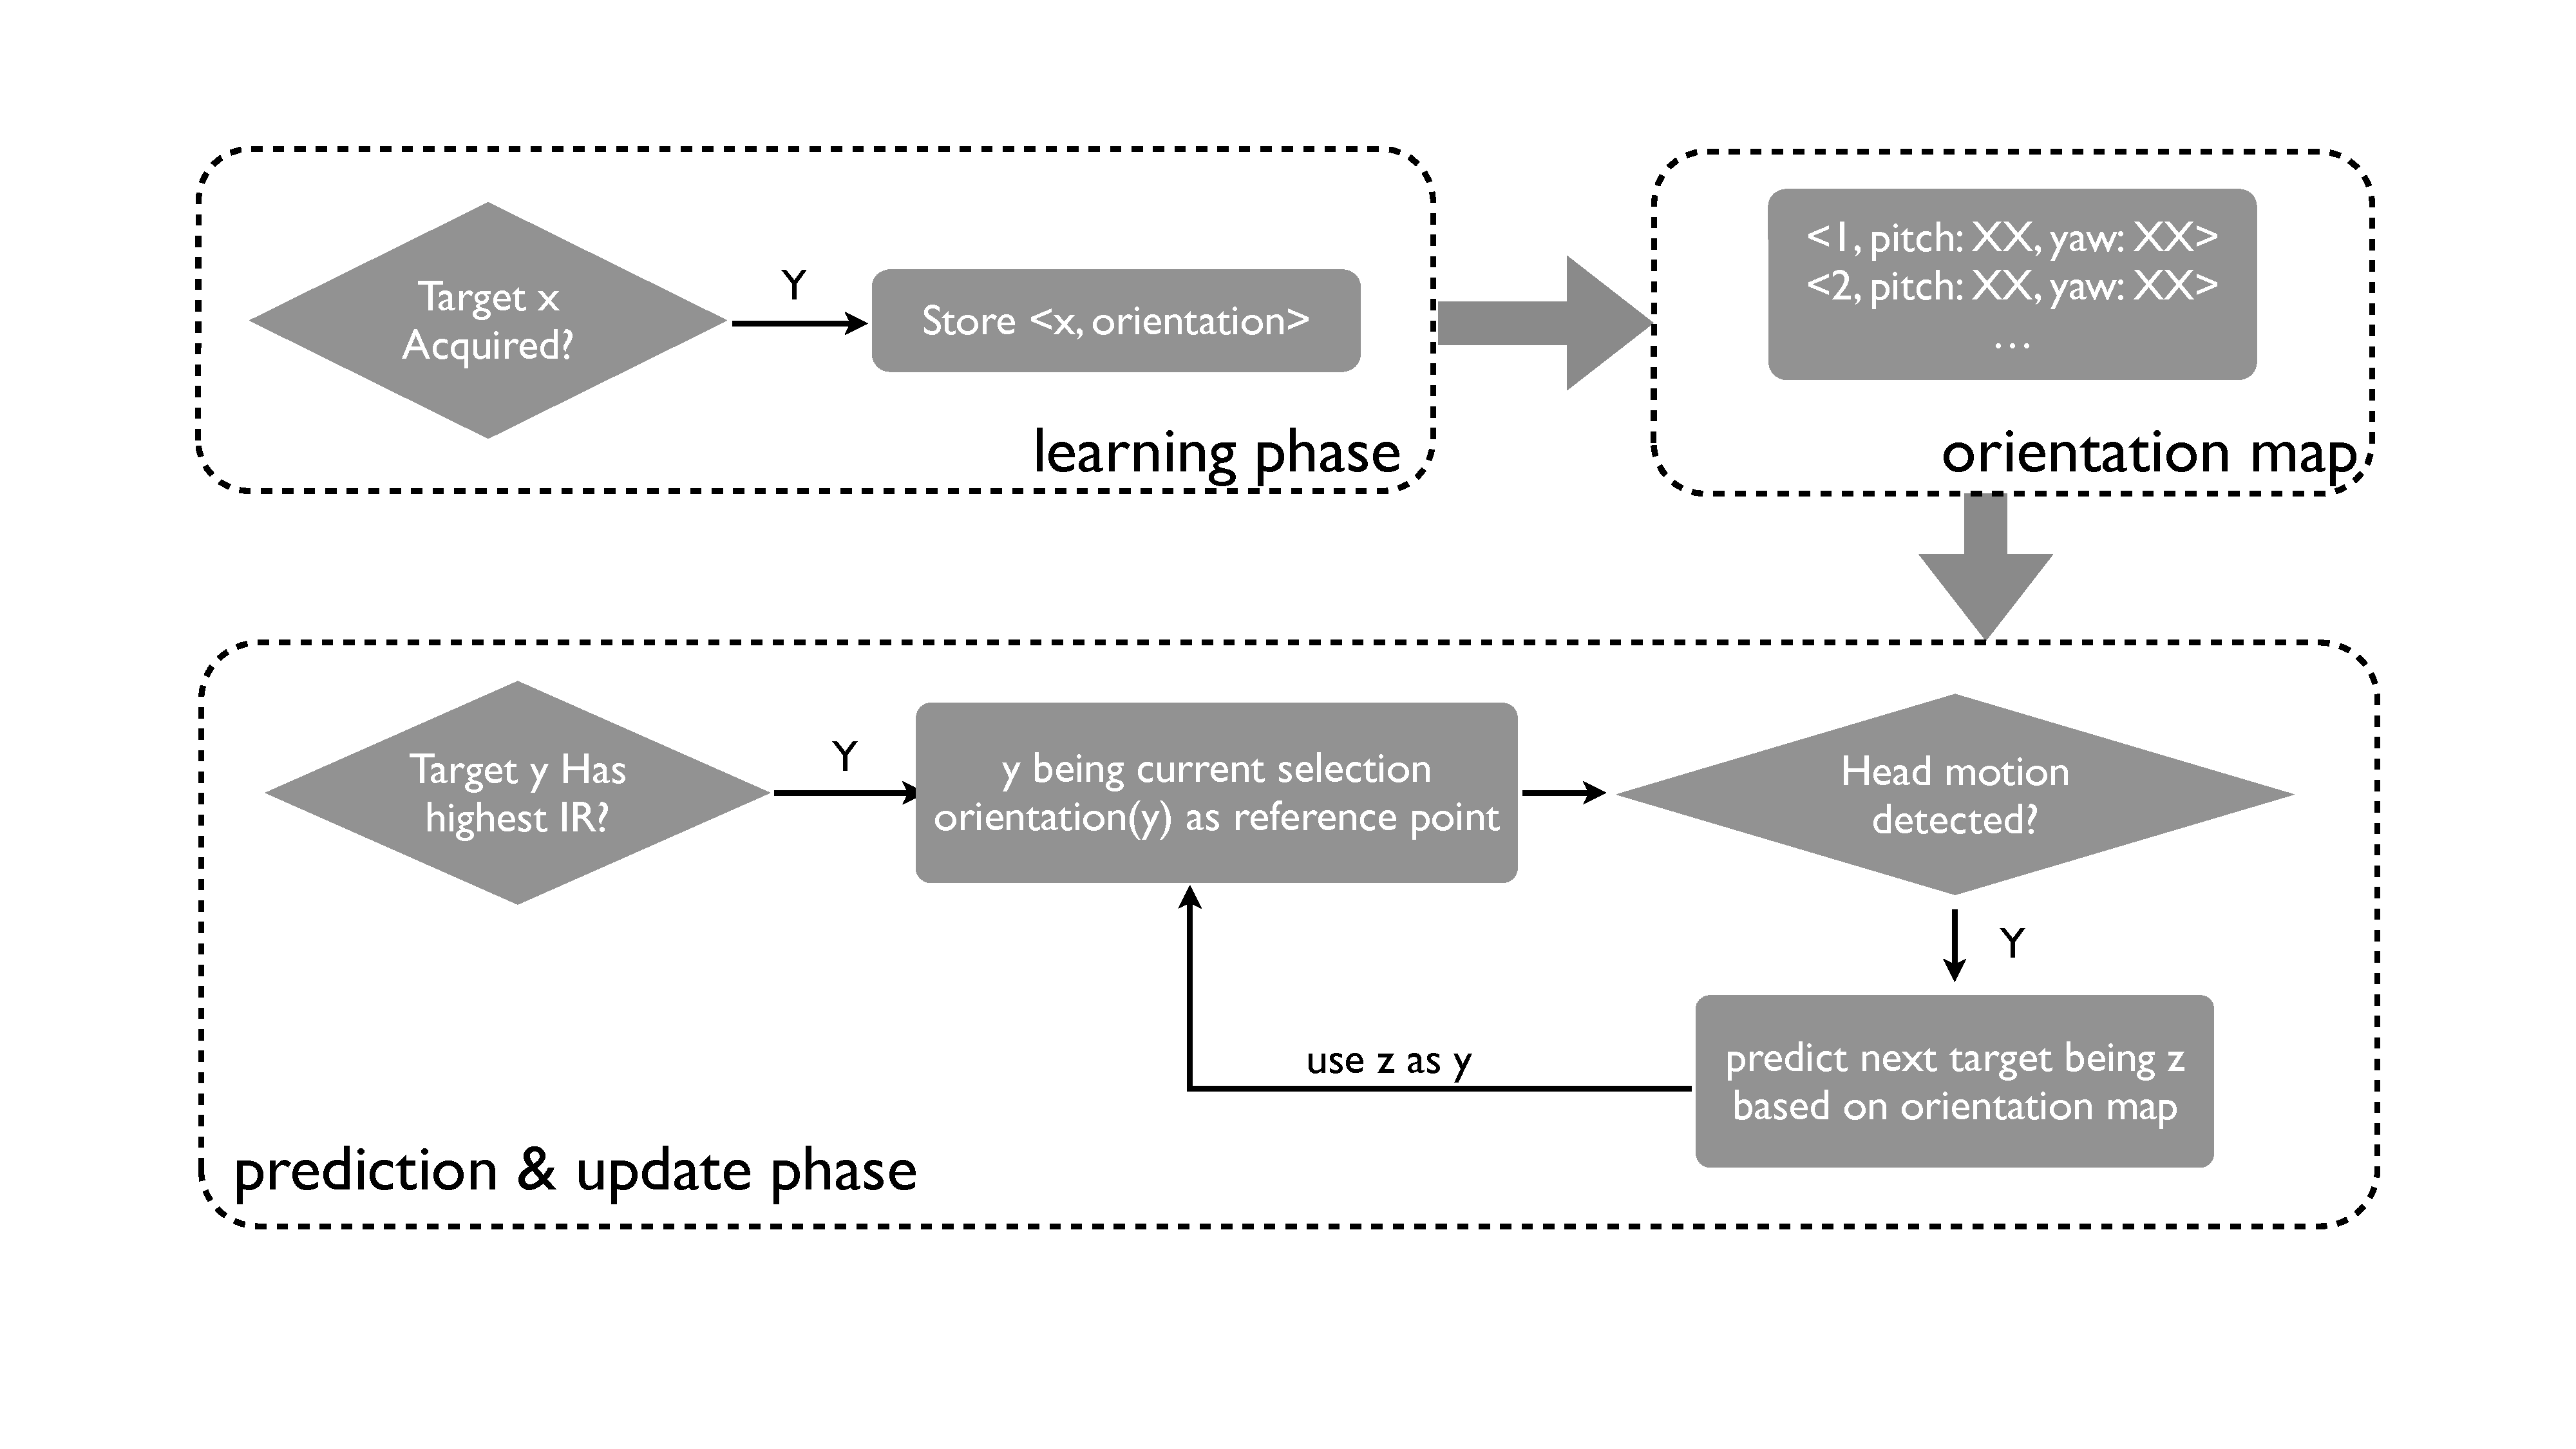
\includegraphics[width=0.95\columnwidth]{figures/third_technique.pdf}
\caption{Our third technique learned each target's absolute orientation and
construct the adjacency map. During the {\em refinement} stage, the prediction
is based on relative changes to a reference point.}
\label{fig:third_technique}
\end{figure}

\begin{figure}[t]
\centering
\includegraphics[width=0.95\columnwidth]{figures/third_principle.png}
\caption{This illustrates that the change of a user's absolution position
doesn't change the relative relationship of physical targets.}
\label{fig:third_principle}
\end{figure}

\changes{After the map is created, the user can enter a quasi-mode for
refinement by holding down on the touchpad. In this quasi-mode, a single selected device
lights up at a time. When the user turns his head in the direction of another
device, the selection (and indicator light) switches to that device. Therefore, the user can move between
devices one at a time with slight head movements. This prediction is
implemented by first calculating the user's direction of head motion, and searching
through the adjacency map for the nearest device in that direction.  To
calculate the direction, we maintain a circular buffer of the last 10 sensor
measurements, passed through a low pass filter. The direction is then
calculated as the difference between the last sample and the first sample.
We use a hysteresis method to avoid spurrious selection changes
--- if the variance of the buffer is below a threshold, we assume no movement has
occurred and do not select another device.}

\subsection{Evaluation}
We evaluated the head motion refinement method through an informal study and
collected qualitative feedback from a subset of 4 users from the Iteration 2
study. In this evaluation, we asked users to cycle through multiple targets using
the new quasi-mode.

The users had strong preferences for the new method of refinement.
\changes{Our observations suggest that each trial became much easier than previous iterations. We
conducted a survey to collect qualitative feedback after the
experiment.} 
On a scale from 1-7, 1 being the least mental effort and
7 being the most mental effort users rated the old technique 4.25 and
the new technique 2 on average. All users indicated a preference for head
movement to list navigation. One user referenced the issue of naming
targets that the list necessitates, preferring the experience of
\studyquote{matching visual cues rather than numbers}.  Another
participant remarked that it \studyquote{just made more sense} and was
a \studyquote{more natural way for demonstrating intentionality}. The
users preferred the new mapping in relation to the whole environment:
\studyquote{it leveraged the spatial sense that I already had just by
using the system}. They were also delighted to avoid list navigation,
which they now called \studyquote{difficult} and \studyquote{painful}.
